\documentclass[8pt]{beamer}
\usetheme{Berlin}
\usecolortheme{seahorse}
\usepackage{sansmathfonts}

\usepackage{amsmath, amssymb, amsthm}
\usepackage{stmaryrd}

\usepackage{tikz}
\usetikzlibrary{positioning}

\title{Denotational Sematics for Recursion in Guarded Type Theory}
\subtitle{{\tiny based on MFPS'15 \textit{A Model of PCF in Guarded Type Theory} by Marco Paviotti, Rasmus Ejlers Møgelberg, and Lars Birkedal}}
\author{Charles Peng}
\institute{Aarhus University}
\date{\today}

\newcommand{\sem}[1]{{[\![ {#1} ]\!]}}
\newcommand{\unit}{\mathbf{unit}}
\newcommand{\bool}{\mathbf{bool}}
\newcommand{\nat}{\mathbf{nat}}
\newcommand{\Nat}{\mathbb{N}}
\newcommand{\Bool}{{\{\mathbf{T},\mathbf{F}\}}}
\newcommand{\Unit}{{\{\ast\}}}
\newcommand{\eqdef}{\triangleq}
\newcommand{\typed}[3]{{{#1}\vdash{#2}\,:\,{#3}}}
\newcommand{\ectx}{\bullet}
\newcommand{\univ}{\mathcal{U}}

\newcommand{\bigstep}{\Downarrow}

\newcommand{\prd}{\mathbin{\text{\texttt{pred}}}}
\newcommand{\suc}{\mathbin{\text{\texttt{succ}}}}
\newcommand{\ifz}{\mathbin{\text{\texttt{ifz}}}}
\newcommand{\ite}{\mathbin{\text{\texttt{ite}}}}
\newcommand{\fix}{\mathbin{\text{\texttt{fix}}}}
\newcommand{\gfix}{\mathbin{\text{\texttt{gfix}}}}
\newcommand{\ret}{\mathbin{\textcolor{bronze}{\text{\texttt{pure}}}}}
\newcommand{\pure}{\mathbin{\textcolor{bronze}{\text{\texttt{next}}}}}
\newcommand{\fmap}{\mathbin{\textcolor{magenta}{\text{\texttt{<\$>}}}}}
\newcommand{\ap}{\mathbin{\textcolor{americanrose}{\text{\texttt{<*>}}}}}

\newcommand{\Y}{\mathbin{\textcolor{brown}{\text{\texttt{Y}}}}}
\newcommand{\Term}{\mathbin{\text{\texttt{Term}}}}
\newcommand{\Value}{\mathbin{\text{\texttt{Value}}}}
\newcommand{\Type}{\mathbin{\text{\texttt{Type}}}}

\newcommand{\later}{{\mathop{\rhd}}}

\newcommand{\RR}[3]{{#2}\,\textcolor{blue}{\mathcal{R}_{#1}}\,{#3}}
\newcommand{\RRd}[3]{{#2}\,\textcolor{blue}{\later\!\mathcal{R}_{#1}}\,{#3}}

\newcommand{\tand}{\land}

\newcommand{\demph}[1]{\textcolor{gray}{#1}}

\definecolor{americanrose}{rgb}{1.0, 0.01, 0.24}
\definecolor{bronze}{rgb}{0.8, 0.5, 0.2}


\begin{document}

\maketitle

\section{Introduction to Denotational Semantics}

\begin{frame}{Flavors of semantics}
	\begin{itemize}
		\item small-step/structural op-sem: how programs evolve during execution
			\begin{equation*}
				\frac{s \to s'}{(\lambda x . e)\, s \to (\lambda x . e)\, s'}
				\qquad
				\frac{\Value\,s}{(\lambda x . e)\, s \to e[s/x]}
			\end{equation*}
		\item big-step/natural op-sem: how to evaluate a program
			\begin{equation*}
				\frac{n \bigstep \underline{0} \quad E_0 \bigstep V_0}{\ifz(n;E_0,E_1)\bigstep V_0}
					\qquad
					\frac{n \bigstep \underline{1\!+m} \quad E_1 \bigstep V_1}{\ifz(n;E_0,E_1)\bigstep V_1}
					\end{equation*}
				\item predicate-transformer / Hoare Logic: what is the necessary condition at each stage of execution
					\begin{equation*}
						\frac{\{P\}e_1\{Q\}\quad\{Q\}e_2\{R\}}{\{P\}e_1;e_2\{R\}}
					\end{equation*}
				\item algebraic laws and equational reasoning
					\begin{equation*}
						f \fmap (g \fmap x) \equiv (f \circ g) \fmap x
						\qquad
						\ret\,f \ap  \ret\,x \equiv \ret(f\,x)
					\end{equation*}
			\end{itemize}
			We will talk about denotational semantics today.
		\end{frame}

\begin{frame}{when it is natural to think about the denotation}
	Regular expressions: $\emptyset$, $\epsilon$, $\{c\}$, $r_1 \cdot r_2$, $r_1|r_2$, $r^*$.\\
	How do we understand \texttt{\^{}cs538 assignment.*grade (F|D)\$}

	\begin{block}{Operational semantics: how to match a string}
		\begin{equation*}
			\frac{}{M(r^*, s) \Rightarrow (\epsilon, s)}
			\qquad
			\frac{M(r,s) \Rightarrow (s_1, t_1) \quad M(r^*,t_1)\Rightarrow (s_2, t_2)}
			{M(r^*, s) \Rightarrow (s_1 \cdot s_2, t_2)}
		\end{equation*}
		Wow, you are a regex engine hacker.
	\end{block}

	\begin{block}{Denotational semantics: what are matched by a pattern}
		\begin{align*}
			\mathcal{M}(r_1 | r_2) &= \mathcal{M}(r_1) \cup \mathcal{M}(r_2)\\
			\mathcal{M}(r^*) &= \bigcup_{n\in\mathbb{N}}\mathcal{M}(r^k) = \fix(\lambda  T . \{\epsilon\} \cup \{s\cdot t \mid s \in \mathcal{M}(r) \land t\in T\})
		\end{align*}
		Oh, we are normal programmers.
	\end{block}

	\textbf{Caveat} the connotation, ``assignments that I have to re-handin'', is out of scope.
\end{frame}

\begin{frame}{Propositional logic as a PL and two semantics for the PL}
	How do we understand a statement in propositional logic? For example, $p\land q \to p$
	\begin{itemize}
		\item Proofs and provability\\
			\begin{itemize}
				\item Transform the sequent with rules. Construct a closed proof tree.
				\item Example: go from $\Gamma, \phi \vdash \psi$ to $\Gamma \vdash \phi \to \psi$.
				\item $\vdash p\land q\to p$ is a theorem: proved by $\to I$ and $\land E_l$.
			\end{itemize}
		\item Interpretations and satisfiability\\
			\begin{itemize}
				\item Assign values to variable. Define the truth table of connectives.
				\item Example: $I\models \phi \land \psi$ iff $I\models\phi$ and $I\models\psi$.
				\item $\models p\land q \to p$ is a tautology: true under all interpretations.
			\end{itemize}
	\end{itemize}
		
	Proofs: how to operationally prove statements. Operational semantics of logics.\\
	Models: what does being true means. Denotational semantics of logics.\\
	
	\vfill
	\begin{block}{desirable aspects of model theory}
		Determining equivalence is often eaiser in denotational semantics.
	\end{block}
\end{frame}


\begin{frame}[allowframebreaks]{The Set-theoretic model of STLC: A recipie you can replicate}
	Types are sets of values
	\begin{align*}
		\sem{\unit} &\eqdef \Unit \\
		\sem{\bool} &\eqdef \Bool \\
		\sem{\nat} &\eqdef \Nat \\
		\sem{\sigma\to \tau} &\eqdef \sem{\sigma}\to\sem{\tau} \\
		\sem{\sigma\times \tau} &\eqdef \sem{\tau} \times \sem{\sigma} \\
		\sem{\sigma + \tau} &\eqdef \sem{\sigma} \uplus \sem{\tau} 
	\end{align*}
	Closed-terms are things that will reduce to a value, but what about open terms?

	\framebreak
	Open terms can be closed by substituting free variables with well-typed values.\\[4ex]

	$\typed{\Gamma}{e}{\tau}$ where the context is $\Gamma = x_1 : \sigma_1, x_2 : \sigma_2, \ldots$
	\begin{enumerate}
		\item A series of terms $v_i$ such that $\typed{\ectx}{v_i}{\sigma_i}$
		\item Substitution to have a closed term $\typed{\ectx}{e[v_1/x_1,\ v_2/x_2,\ \ldots]}{\tau}$
		\item The term $e[v_1/x_1,\ v_2/x_2,\ \ldots]$ will reduce to a value in $\sem{\tau}$
	\end{enumerate}
	\vspace{3ex}
	$\sem{\typed{\Gamma}{e}{\tau}}$ is a function from $\sem{\Gamma} = \sem{\sigma_1}\times \sem{\sigma_2}\times \ldots$ to $\sem{\tau}$\\[3ex]
	Specifically $\sem{\typed{\ectx}{e}{\tau}}$ is a function from $\Unit$ to $\sem{\tau}$

	\framebreak
	Interpret type judgements by induction on the type derivation.

	\begin{itemize}
		\item $\typed{\Gamma}{x_i}{\sigma_i}$ a variable references is a projection
			\begin{align*}
				\sem{\typed{x_1:\sigma_1,\ldots x_n:\sigma_n}{x_i}{\sigma_i}} &\eqdef \pi_i & \sem{\sigma_1}\times \sem{\sigma_2} \times \cdots \sem{\sigma_n} \to \sem{\sigma_i}
			\end{align*}
		\item $\typed{\Gamma}{M\,N}{\tau}$ an application is a S-combinator
			\begin{align*}
				f &= \sem{\typed{\Gamma}{M}{\sigma\to \tau}} & \sem{\Gamma}\to (\sem{\sigma} \to \sem{\tau}) \\
				g &= \sem{\typed{\Gamma}{N}{\sigma}}      & \sem{\Gamma}\to \sem{\sigma}         \\
				\sem{\typed{\Gamma}{M\ N}{\tau}} &\eqdef S\,f\,g = \lambda \gamma . f\,\gamma\,(g\,\gamma) & \sem{\Gamma}\to\sem{\tau}
			\end{align*}
		\item $\typed{\Gamma}{\lambda x^\sigma . e}{\sigma\to \tau}$ a $\lambda$-abstraction is currying
			\begin{align*}
				f &= \sem{\typed{\Gamma, x:\sigma}{e}{\tau}} & \sem{\Gamma}\times \sem{\sigma} \to \sem{\tau} \\
				\sem{\typed{\Gamma}{\lambda x^\sigma . e}{\sigma\to\tau}} &\eqdef \lambda \gamma . \lambda a . f\ (\gamma,a) & \sem{\Gamma} \to \sem{\sigma} \to \sem{\tau}
			\end{align*}
	\end{itemize}
% SLOGAN: eta for now, theta for later, delta for delay
	\framebreak
	Prove some theorems
	\begin{itemize}
		\item soundness: $M =_{\beta\eta} N \implies \sem{\typed{\Gamma}{M}{\tau}}=\sem{\typed{\Gamma}{N}{\tau}}$\\
			Straight forward induction:
			\begin{enumerate}
				\item weakening lemma to handle context extension
				\item substitution lemma $\sem{\typed{\Gamma}{M[N/x]}{\tau}} = \sem{\typed{\Gamma}{(\lambda x^\sigma . M)N}{\tau}}$
				\item congruence lemma
				\item beta-reduction/eta-expansion preserves denotational equivalence
			\end{enumerate}
		\item adequacy: $\sem{\typed{\Gamma}{M}{\tau}}=v \implies M =_{\beta\eta} \underline{v}$
			\begin{itemize}
				\item define a type-index logical relation that captures hereditary normalization. $e\ R_T\ \sem{u}$
				\item application of related things are related
				\item subject expansion
				\item substitution lemma
				\item subject reduction
				\item fundamental lemma: closing-substitution for well-typed terms is in the relation
			\end{itemize}
		\item completeness: PL folks don't care about this\footnote{FYI, search for Henkin models}
		\item full abstraction: $M =_{\beta\eta} N \iff \sem{\typed{\Gamma}{M}{\tau}}=\sem{\typed{\Gamma}{N}{\tau}}$\\
			out of scope.
	\end{itemize}
\end{frame}

\begin{frame}{The problem of generalizability}
	Denotational semantics is natural!\\
	Set-theoretic model cannot accomodate general recursion.
	\begin{itemize}
		\item mutable states
		\item general references
		\item parametric polymorphism
		\item non-local jumps e.g. exceptions, call/cc
		\item effects e.g. input/output
		\item ...
	\end{itemize}

	\vfill
	Solution: interpret program in semantic domains with rich structures
	\begin{itemize}
		\item More proof obligations: constructions respect the domain structure.
		\item The way out: construct domains in metatheory $\implies$ domain inside the metatheory
		\item The type theory automatically guarantees the constructions can be accomodated.
	\end{itemize}
\end{frame}

\section{Review of Guarded Type Theory}
\begin{frame}{more fixed point constructions that make sense}
	Explicit solution of least fixed point is often unnecessary.\\
	We only care about unfolding.\\
	\begin{equation*}
		Y=\fix\, F \cong F(Y)
		\qquad \qquad
		Y
		\stackrel{\text{unfold}}{\longrightarrow}
		F(Y)
	\end{equation*}
	\begin{itemize}
		\item dynamic system: $F(X) = X$
		\item stream $F(X) = A \times X$
		\item deterministic automata\footnote{may have infinite states} $F(X) = 2 \times X^A$
		\item deterministic automata, partial transition function $F(X) = 2 \times {(1 + X})^A$
		\item non-deterministic automata $F(X) = 2 \times {\mathcal{P}(X)}^A$
	\end{itemize}

	\vspace{3ex}

	We will want things that are not even co-algebra!
\end{frame}
\begin{frame}{time in the metatheory}
	\textbf{Intuition} $\later A$ is same as $A$ but available only in the next step.
	\begin{itemize}
		\item a new modality $\later$ later
		\item applicative functor
			\begin{itemize}
				\item $\pure : A \to \later A$
				\item $\ap : \later (A \to B) \to \later A \to \later B$
				\item Algebraic laws. Notably $(\pure\, f)\,\ap\,(\pure\, x) = \pure\,(f\, x)$
				\item Induced $\fmap : (A \to B) \to \later A \to \later B$ where $f \fmap x \eqdef (\pure\,f)\,\ap\, x$
			\end{itemize}
		\item delayed substitution
			\begin{itemize}
				\item Formation $\typed{\Gamma}{f}{\Pi(x:A) . B}$ and $\typed{\Gamma}{t}{\later A}$ then $\typed{\Gamma}{f\,\ap\,t}{\later [x \gets t]. B}$
				\item Computation $\later [x\gets \pure\, t] . B \equiv \later B[u/x]$
			\end{itemize}
		\item guarded fixed point combinator $\gfix : (\later A \to A) \to A$
			\begin{equation*}
				\gfix (F) \equiv \fix (F\circ \pure) \equiv F (\pure (\gfix(F))) \equiv {(F \circ \pure)}^n (\gfix (F))
			\end{equation*}
			Access to the recursive structure is stratified.
	\end{itemize}
\end{frame}
\begin{frame}[allowframebreaks]{later algebra}
	$\later$-algebra $(A,\theta_A)$ where $A: \univ$ and $\theta_A : \later A \to A$\\

	\begin{block}{delayed computation}
		\begin{enumerate}
			\item Given $a:A$, make it available later $\pure\,a : \later A$
			\item Pull delayed value back $\theta (\pure\, a) : A$
			\item $\delta \eqdef \theta \circ \pure : A \to A$ adds one time step to the computation
		\end{enumerate}
	\end{block}

	\begin{block}{every later algebra has a bottom element}
		\begin{equation*}
			\bot \eqdef \gfix (\theta)
			\equiv \theta (\pure (\gfix (\theta)))
			\equiv \delta (\bot)
		\end{equation*}
	\end{block}

	\newcommand{\Stm}{\mathbin{\text{\texttt{Stream}}}_A}
	A type sort / an universe is a $\later$-algebra: define datatypes with guarded recursion
	\begin{equation*}
		\Stm \equiv \gfix(\lambda X . A \times X) \cong A \times \later \Stm
	\end{equation*}
\end{frame}
\begin{frame}[allowframebreaks]{Types are step-indexed spaces}
	\begin{tabular}{lll}
		Types & propositions & $P_i$ to be satisfied, at stage $i$\\
		Program & proofs & witness $\vdash x_i : P_i$, at stage $i$\\
	\end{tabular}
	\begin{center}
		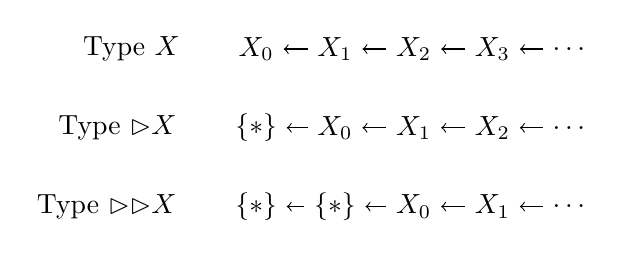
\begin{tikzpicture}[node distance=1cm]
			% Nodes for Diagram X
			\node (X0) {$X_0$};
			\node (X1) [right of=X0] {$X_1$};
			\node (X2) [right of=X1] {$X_2$};
			\node (X3) [right of=X2] {$X_3$};
			\node (dots) [right of=X3] {$\dots$};
			% Arrows for Diagram X
			\draw[<-] (X0) -- (X1);
			\draw[<-] (X1) -- (X2);
			\draw[<-] (X2) -- (X3);
			\draw[<-] (X3) -- (dots);
			% Nodes for Diagram LX (below)
			\node (star0) [below of=X0] {$\{\ast\}$};
			\node (LX0) [right of=star0] {$X_0$};
			\node (LX1) [right of=LX0] {$X_1$};
			\node (LX2) [right of=LX1] {$X_2$};
			\node (dots2) [right of=LX2] {$\dots$};
			% Arrows for Diagram LX
			\draw[<-] (star0) -- (LX0);
			\draw[<-] (LX0) -- (LX1);
			\draw[<-] (LX1) -- (LX2);
			\draw[<-] (LX2) -- (dots2);
			% Nodes for Diagram LLX (below)
			\node (star1) [below of=star0] {$\{\ast\}$};
			\node (LLX0) [right of=star1] {$\{\ast\}$};
			\node (LLX1) [right of=LLX0] {$X_0$};
			\node (LLX2) [right of=LLX1] {$X_1$};
			\node (dots3) [right of=LLX2] {$\dots$};
			% Arrows for Diagram LLX
			\draw[<-] (star1) -- (LLX0);
			\draw[<-] (LLX0) -- (LLX1);
			\draw[<-] (LLX1) -- (LLX2);
			\draw[<-] (LLX2) -- (dots3);
			% Labels
			\node[left=0.5cm of X0] {Type $X$};
			\node[left=0.5cm of star0] {Type $\later X$};
			\node[left=0.5cm of star1] {Type $\later \later X$};
		\end{tikzpicture}
	\end{center}

	\framebreak

	% \begin{itemize}
	% 	\item At stage $0$, $P_X^0$ is satisfied
	% 	\item At stage $1$, $P_X^1$ is satisfied
	% 	\item $\cdots$
	% 	\item At stage $k$, $P_X^k$ is satisfied
	% \end{itemize}
	% Interpretation of later $\sem{\later X} = (\Unit, P_X^0, P_X^1,\ldots)$
	% \begin{itemize}
	% 	\item At stage $0$, nothing is required
	% 	\item At stage $1$, $P_X^0$ is satisfied
	% 	\item $\cdots$
	% 	\item At stage $k$, $P_X^{k-1}$ is satisfied
	% \end{itemize}
	% Other constructs e.g. $\times$, $\uplus$, $\Pi$, $\Sigma$ are interpreted naturally.\\
	%
	% \framebreak
	% A proof $x:X$ at stage $i$, provide at witness of $P_X^i$.\\
	% A delayed proof $\delta(x) : X$ at stage $i$, provide witness of stage $i-1$.
	%
	% \begin{itemize}
	% 	\item At state $0$, $\bot \equiv \delta^1( \bot )$ any conclusion has to be made at stage $1$
	% 	\item At state $1$, $\bot \equiv \delta^2( \bot )$ any conclusion has to be made at stage $2$
	% 	\item $\cdots$
	% 	\item At state $k$, $\bot \equiv \delta^{k+1}( \bot )$ any conclusion has to be made at stage $k+1$
	% \end{itemize}
	% This is a computation that always with hold the result. $(\Unit,\Unit,\Unit,\Unit,\ldots)$
\end{frame}


\section{A domain of potentially non-terminating computation}
\begin{frame}[allowframebreaks]{the lifting monad}
	A free $\later$-algebra
	\begin{equation*}
		L_A \eqdef \gfix (\lambda X . A + X) \cong A + \later L_A
	\end{equation*}
	\begin{itemize}
		\item either $\eta(a)$ where $a:A$
		\item or $\theta(x')$ where $x':\later L_A$
	\end{itemize}

	\begin{center}
		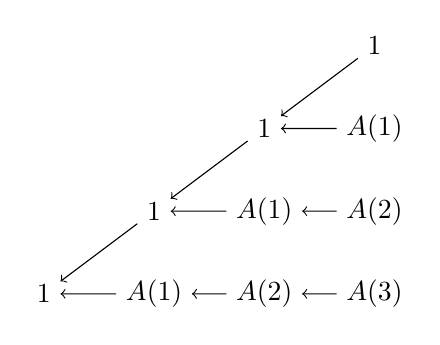
\begin{tikzpicture}[node distance=1cm, scale=0.7]
			\def\n{3}
			% Nodes
			\foreach \i in {0,...,\n} {
				\foreach \j in {0,...,\i} {
					% compute y coordinate
					\pgfmathsetmacro{\y}{-\i*1.5}
					\pgfmathsetmacro{\x}{(\j-\i)*2}

					% choose text
					\ifnum\i=0
						\ifnum\j=0
							\node (n-\i-\j) at (\x,\y) {$1$};
						\else
							\node (n-\i-\j) at (\x,\y) {+};
						\fi
					\else
						\ifnum\j=0
							\node (n-\i-\j) at (\x,\y) {$1$};
						\else
							\node (n-\i-\j) at (\x,\y) {$A(\j)$};
						\fi
					\fi
				}
			}

			% horizontal arrows
			\foreach \i in {1,...,\n} {
				\foreach \j in {1,...,\i} {
					\pgfmathtruncatemacro{\jprev}{\j-1}
					\draw[<-] (n-\i-\jprev) -- (n-\i-\j);
				}
			}

			% diagonal arrows
			\foreach \i in {1,...,\n} {
				\pgfmathtruncatemacro{\iprev}{\i-1}
				\draw[<-] (n-\i-0) -- (n-\iprev-0);
			}
		\end{tikzpicture}
	\end{center}

	\framebreak
	The natural choice for modeling potentially diverging computation.
	\begin{itemize}
		\item An already done computation: $\eta(v)$
		\item A computation that terminates in $1$ step: $\theta(\pure(v)) = \delta(v)$
		\item A computation that terminates in $2$ step: $\theta(\pure (\theta (\pure (v)))) = \delta^2(v)$
	\end{itemize}
	The bottom element of $L_A$: $\bot_{L_A} \eqdef \gfix (\theta)$
	\begin{itemize}
		\item Unfold $1$: $\delta^1$ of $\bot$
		\item Unfold $2$: $\delta^2$ of $\bot$
		\item $\cdots$
		\item Unfold $k$: $\delta^k$ of $\bot$
	\end{itemize}
\end{frame}

\begin{frame}{A mnemonic}
	\begin{itemize}
		\item $\eta$ for now
		\item $\theta$ for future
		\item $\delta$ for delay
	\end{itemize}
\end{frame}

\begin{frame}{$\later$-algebra is closed under function type formation}
	From $(A,\theta_A)$ and $(B,\theta_B)$, build $(A\to B, \theta_{A\to B})$
	\begin{enumerate}
		\item Construct $A\to B$ from $f : \later (A\to B)$
		\item Abstract over $x : A$. Make it available later $\pure(x) : \later A$.
		\item Apply the function later $f \,\ap\,\pure(x) : \later B$
		\item Use $\theta_B$ to embed the delayed value.
	\end{enumerate}
	\begin{equation*}
		\theta_{A\to B} \eqdef \lambda (f : \later (A \to B)) (x : \later A) \,.\, \theta_B(f\,\ap\,\pure\,x)
	\end{equation*}

	\vspace{8ex}

	A family of $\later$-algebras formed by lifting monads and functions.\\
	A domain for ``potentially terminating computations that may result in a value''.
\end{frame}


\section{A guarded recursion semantics for PCF}
\subsection{Interpretation of PCF in the domain}
\begin{frame}{Interpreation of types}

	Interpret base types as lifting monads:
	\begin{equation*}
		\sem{\unit} \eqdef L_{\Unit}
		\qquad \sem{\bool} \eqdef L_{\Bool}
		\qquad \sem{\nat} \eqdef L_{\Nat}
	\end{equation*}
	Interpret function type as functions between semantic domains
	\begin{equation*}
		\sem{S \to T} \eqdef \sem{S} \to \sem{T}
	\end{equation*}

	Semantic domain of every type is a $\later$-algebra
	\begin{itemize}
		\item Base types: $\theta_{\sem{\nat}} : \later L_{\Nat} \to L_{\Nat}$
		\item Function types: $\theta_{\sem{S}\to \sem{T}}$ build from $\theta_{\sem{S}}$ and $\theta_{\sem{T}}$
	\end{itemize}
\end{frame}
\begin{frame}{Interpretation of type judgements}
	$\fbox{$\sem{\typed{\Gamma}{M}{\tau}}(\gamma)$}$ \quad ``The denotation of $M$ given interpreation of free variables in $\gamma$''
	\begin{align*}
		\demph{\sem{\typed{\Gamma, x_i:\sigma_i,\Delta}{x_i}{\sigma_i}}(\gamma)} &\demph{\eqdef \pi_i} \\
		\demph{\sem{\typed{\Gamma}{\lambda x . M}{\sigma\to\tau}}(\gamma)} &\demph{\eqdef \lambda x^{\sem{\sigma}}.\sem{\typed{\Gamma,x:\sigma}{M}{\tau}}(\gamma,x)} \\
		\demph{\sem{\typed{\Gamma}{M\ N}{\tau}}(\gamma)} &\demph{\eqdef \sem{\typed{\Gamma}{M}{\sigma\to\tau}}(\gamma)(\sem{\typed{\Gamma}{N}{\sigma}}(\gamma))} \\
		\sem{\typed{\Gamma}{\underline{n}}{\nat}}(\gamma) &\eqdef \eta(n) \\
		\sem{\typed{\Gamma}{\prd\, M}{\nat}}(\gamma) &\eqdef (-1) \fmap \sem{\typed{\Gamma}{M}{\nat}}(\gamma) \\
		\sem{\typed{\Gamma}{\suc\, M}{\nat}}(\gamma) &\eqdef (+1) \fmap \sem{\typed{\Gamma}{M}{\nat}}(\gamma) \\
	\sem{\typed{\Gamma}{\ifz\, M\,N_0\,N_1}{\tau}}(\gamma) &\eqdef \widehat{\ifz}(\sem{\typed{\Gamma}{M}{\nat}}(\gamma); \sem{\typed{\Gamma}{N_0}{\tau}}(\gamma),\sem{\typed{\Gamma}{N_1}{\tau}}(\gamma)) \\
		\sem{\typed{\Gamma}{\Y\,M}{\tau}}(\gamma) &\eqdef \gfix (\lambda x^{\later \sem{\tau}}\ .\ \theta_{\sem{\tau}}(\pure (\sem{\typed{\Gamma}{M}{\tau\to\tau}}(\gamma)) \ap x)) \\
	\end{align*}
\end{frame}
\begin{frame}{Unfold in object language is delayed evaluation in metatheory}
	\begin{equation*}
		\sem{\typed{\Gamma}{\Y\,M}{\tau}} = \delta \circ \sem{\typed{\Gamma}{M\,(\Y\,M)}{\tau}}
	\end{equation*}
	To show
	\begin{equation*}
		\sem{\typed{\Gamma}{\Y\,M}{\tau}}(\gamma) = \theta_{\sem{\tau}} (\pure (\sem{\typed{\Gamma}{M\,(\Y\,M)}{\tau}}(\gamma)))
	\end{equation*}
	Proof
	\begin{align*}
		\mathrm{LHS} & = \gfix (\lambda x^{\later \sem{\tau}}\ .\ \theta_{\sem{\tau}}(\pure (\sem{\typed{\Gamma}{M}{\tau\to\tau}}(\gamma)) \ap x))        \\
					 & = \theta_{\sem{\tau}}\left(\pure (\sem{\typed{\Gamma}{M}{\tau\to\tau}}(\gamma)) \ap \pure\, \mathrm{LHS}\right)                    \\
					 & = \theta_{\sem{\tau}}\left(\pure (\sem{\typed{\Gamma}{M}{\tau\to\tau}}(\gamma)(\mathrm{LHS})\right)                                \\
		\mathrm{RHS} & = \theta_{\sem{\tau}}\left(\pure\ \sem{\typed{\Gamma}{M}{\tau\to\tau}}(\gamma) (\sem{\typed{\Gamma}{\Y\,M}{\tau}}(\gamma)) \right) \\
					 & = \theta_{\sem{\tau}}\left(\pure\ \sem{\typed{\Gamma}{M}{\tau\to\tau}}(\gamma) (LHS) \right)
	\end{align*}
\end{frame}
	% TODO: revise this to reflect proof sketch

\begin{frame}{Step-indexing big-step operational semantics}
	$\fbox{$M \bigstep^k Q$}$ \quad ``$\typed{\ectx}{M}{\tau}$ reduces to a value $v$ in $l<k$ steps satisfying $Q(v,k-l)$''.


	\begin{align*}
		\demph{v \bigstep^k Q}                & \demph{\eqdef Q(v,k)}                                                                                                 \\
		\demph{\prd\,M \bigstep^k Q}          & \demph{\eqdef M \bigstep \lambda x . \lambda l . \Sigma n . x = \underline{n} \tand Q(\underline{n-1},l)}             \\
		\demph{\suc\,M \bigstep^k Q}          & \demph{\eqdef M \bigstep \lambda x . \lambda l . \Sigma n . x = \underline{n} \tand Q(\underline{n+1},l)}             \\
		\demph{\ifz\,M\,N_0\,N_1\bigstep^k Q} & \demph{\eqdef M \bigstep \lambda x . \lambda l . \widehat{\ifz}(x ; N_0 \bigstep^l Q, N_1 \bigstep^l Q)}              \\
		\demph{M\,N \bigstep^k Q}             & \demph{\eqdef M\bigstep^k \lambda v . \lambda l . \Sigma x L . v = \underline{\lambda x.L} \tand L[N/x] \bigstep^l Q} \\
		\Y\,M \bigstep^k Q                    & \eqdef \Sigma k' . k = 1\!+k' \land \later (M\, (\Y\,M) \bigstep^{k'} Q)                                              \\
	\end{align*}

	Short-hand notation: $M \bigstep^k_o v = M\bigstep^k \lambda u . \lambda l . l = 0 \tand u = v$.
\end{frame}

\subsection{Soudness proof sketch}
\begin{frame}{Soundness of denotational semantics w.r.t. big-step operational semantics}
	The denotation of operationally equivalent closed-terms coincide.
	\begin{equation*}
		M \bigstep^k_o v
		\implies
		\sem{\ectx \vdash M : \tau} = \delta^k \circ \sem{\typed{\ectx}{v}{\tau}}
	\end{equation*}
	\begin{enumerate}
		\item Unfold-counting small-step op-sem $M \Rightarrow^k v$
		\item Substitution in object language $\iff$ composition of denotation
		\item Unfold-free reduction preserves denotation
		\item Each unfold step introduce a delay
		\item Synchronization: op-sem reduction sequence dictates the evaluation of denotation
	\end{enumerate}
\end{frame}

\subsection{Adequacy proof sketch}
\begin{frame}{Adequacy of denotational semantics w.r.t. big-step operational semantics}
	Evaluation in the denotational domain is big-step evaluation.
	\begin{equation*}
		\sem{\ectx \vdash M : \nat}(\ast) = \delta^k \sem{\typed{\ectx}{v}{\nat}}(\ast)
		\implies
		M \bigstep^k_o v
	\end{equation*}
\end{frame}
\begin{frame}{Logical relation proof method}
	Strengthen the induction hypothesis, so it becomes inductive:
	\begin{itemize}
		\item preserved under congruent reduction
		\item preserved under substitution
		\item preserved under unfolding of $\Y$
	\end{itemize}
\end{frame}
\begin{frame}{The logical relation}
	$\fbox{$\mathcal{R}_{\tau} : \sem{\tau} \to \Term \to \univ$}$ \quad ``associating a term and a denotation''
	\begin{align*}
		\RR{\nat}{\eta(v)}{M}        & \eqdef M \bigstep^0_o v                                                                                        \\
		\RR{\nat}{\theta_\nat(r)}{M} & \eqdef \Sigma M_0^{\Term},M_1^{\Term}\ .\ M\to^0_* M_0 \tand M_0 \to^1 M_1 \tand \RRd{\nat}{r}{M_1}            \\
		\RR{\sigma\to\tau}{f}{M}     & \eqdef \Pi\, \alpha^{\sem{\sigma}},N^{\Term}\ .\ \RR{\sigma}{\alpha}{N} \implies \RR{\tau}{f(\alpha)}{(M\, N)} \\
	\end{align*}

	Delayed relation:
	\begin{equation*}
		\RRd{\nat}{\alpha}{M} \eqdef \later [x\gets \alpha, y\gets M] . (\RR{\nat}{x}{y})
	\end{equation*}
	Notably
	\begin{equation*}
		\RRd{\nat}{\pure\,\alpha}{\pure\,M} \eqdef \later (\RR{\nat}{\alpha}{M})
	\end{equation*}
\end{frame}

\begin{frame}{application lemma}
	\begin{equation*}
		\RRd{\sigma\to \tau}{f}{\pure\, M}
		\land
		\RRd{\sigma}{r}{\pure\, N}
		\implies
		\RRd{\tau}{f \ap r}{\pure\, (M\,N)}
	\end{equation*}
\end{frame}

\begin{frame}{subject expansion: one unfold}
	For $M\to^1 N$ reduction by unfolding\footnote{either by a top-level unfolding or a congruence reduction} $\Y$
	\begin{equation*}
		\RRd{\tau}{\alpha}{\pure N}
		\implies
		\RR{\tau}{\theta(\alpha)}{M}
	\end{equation*}
\end{frame}

\begin{frame}{subject expansion\&reduction: unfold-free step}
	For $M \to^0 N$ reduction without unfolding $\Y$
	\begin{equation*}
		\RR{\tau}{\alpha}{M}
		\iff
		\RR{\tau}{\alpha}{N}
	\end{equation*}
\end{frame}


\begin{frame}{fundamental lemma}
	\begin{itemize}
		\item Open term $\typed{\Gamma}{e}{\tau}$ where $\Gamma = x_1 : \sigma_1,\ldots,x_n:\sigma_n$
		\item Instantiation $\RR{\sigma_i}{\alpha_i}{s_i}$ for $i=1,2,\ldots,n$
		\item Related closing substitution $\RR{\tau}{\sem{\typed{\Gamma}{t}{\tau}}(\alpha_1,\ldots,\alpha_n)}{t[s_1/x_1,\ldots,s_n/x_n]}$
	\end{itemize}
\end{frame}

\begin{frame}{closing up the proof}
	Recall adequacy:
	\begin{equation*}
		\sem{\ectx \vdash M : \nat}(\ast) = \delta^k \sem{\typed{\ectx}{v}{\nat}}(\ast)
		\implies
		M \bigstep^k_o v
	\end{equation*}
	By fundamental lemma, $\RR{\nat}{\delta^k(v)}{M}$\\
	Induction on $k$:
	\begin{itemize}
		\item $\RR{\nat}{\delta^0(v)}{M}$ by definition $M \bigstep^0_o v$
		\item $\RR{\nat}{\theta(\pure(\delta^k(v)))}{M}$
			exists $M_0,M_1$ such that $M\to^0_* M_0$, $M_0\to^1 M_1$, and
			\begin{equation*}
				\RRd{\nat}{\pure (\delta^k(v))}{\pure(M_1)}
				\implies
				\later ( \RR{\nat}{\delta^k(v)}{M_1} )
				\implies
				\later ( M_1\bigstep^k_o v )
			\end{equation*}
			Chain them up $M \to^0_* M_0\to^1 M_1$ and $\later (M_1\bigstep^k_o v)$: $M \bigstep^{1\!+k}_o v$
	\end{itemize}
\end{frame}

\section{Conclusion}
\begin{frame}{Review \& Prospect}
	What we have seen:
	\begin{itemize}
		\item Time steps of metatheory level reasoning.
		\item Guarded recursion $(\later A \to A)\to A$: $\gfix(F) \equiv (F\circ \pure)\gfix(F)$
		\item The free $\later$-algebra, the lifting monad, $L_A \cong L_A + \later L_A$
		\item Synchronization: $\Y\,M\to^1 M\,(\Y\,M)$ $\iff$ $\sem{\Y\,M} = \delta \circ \sem{M\,(\Y\,M)}$
		\item Yet another logical relation proof for adequacy.
	\end{itemize}
	\vspace{4ex}
	Moral of the story:\\

	\textbf{From} Semantic domain formalized in a metatheory\\
	\textbf{To} Semantic domain baked into the metatheory\\
	\vspace{4ex}

	The efforts of developing advanced type theories will be paid out\\
\end{frame}

\end{document}
